
%------------------------------------------------------------------------
\begin{frame}
	\frametitle{Derivation}
	\begin{block}{Definition}
		\textbf{Derivation} is the process of extracting ordered segments from rows in order to generate new compositional materials. It dates back to the Second Viennese School.
	\end{block}
	\begin{block}{Motivation}
		\begin{itemize}
		\item The choice of a particular segment is an important compositional decision, as it establishes motivic material.
		\item It introduces complementary harmonic regions, one given by the segment, the other given by its set complement.
		\item It maintains motivic coherence under the chosen segment, while producing contrasting harmonic regions.
		\item It presents an opportunity for exploring syntax.
	\end{itemize}
	\end{block}
\end{frame}

%------------------------------------------------------------------------
\begin{frame}
	\frametitle{Derivation with the Retrograde}
	\begin{block}{Example}%\begin{example}
		Create a $2 \times 24$ array where the first row is $S$ followed by $\R(S)$, and the second row is initially undefined.
		\begin{equation*}
		\begin{adjustbox}{width=\textwidth}
			$\left[\begin{array}{cccccccccccc|cccccccccccc}
		10 & 2 & 3 & 0 & 5 & 7 & 4 & 6 & 9 & 8 & 1 & 11 & 11 & 1 & 8 & 9 & 6 & 4 & 7 & 5 & 0 & 3 & 2 & 10 \\
			. & . & . & . & . & . & . & . & . & . & . & . & . & . & . & . & . & . & . & . & . & . & . & .
			\end{array}\right]$
		\end{adjustbox}
		\end{equation*}
		Choose an arbitrary segment, and separate it from the the top row by placing in in the bottom row.
		\begin{equation*}
		\begin{adjustbox}{width=\textwidth}
			$\left[\begin{array}{cccccccccccc|cccccccccccc}
			. & 2 & 3 & . & . & . & 4 & 6 & 9 & 8 & 1 & 11 & . & . & . & . & . & . & 7 & 5 & 0 & . & . & 10 \\
			10 & . & . & 0 & 5 & 7 & . & . & . & . & . & . & 11 & 1 & 8 & 9 & 6 & 4 & . & . & . & 3 & 2 & .
			\end{array}\right]$
		\end{adjustbox}
		\end{equation*}
		The row $V = \{ 2, 3, 4, 6, 9, 8, 1, 11, 7, 5, 0, 10 \}$ is a row derived from $S$, where the ordered segment $\{ 10, 0, 5, 7 \}$ in $S$ is preserved by $\R(V)$.
	\end{block}%\end{example}
\end{frame}

%------------------------------------------------------------------------
\begin{frame}
	\frametitle{Producing Syntax from Derivation}
	\begin{block}{Example}
		Find an operation that makes the chosen segment invariant. It is easily checked that $S_1 = \{ 10, 0, 5, 7 \} = \R\T_5\I(S_1)$. Write an extended combination array $[S \; | \; \R(S) \; | \; \R\T_5\I(S) \; | \; \T_5\I(S_1)]$. In the extended array, the segment $S_1$ would be preserved, but the row derived from $\R\T_5\I(S)$ would not be a transform of $V$. If the set complement of $S_1$ in $V$ were parsed to produce more than one harmonic region, then the complement of $S_1$ under this new derived row would produce different harmonic regions.
	\end{block}
\end{frame}

%------------------------------------------------------------------------
\begin{frame}
	\frametitle{Derivation in Berg's \emph{Lulu}}
	\begin{block}{Example}
		The basic row used by Berg is $S = \{ 10, 2, 3, 0, 5, 7, 4, 6, 9, 8, 1, 11 \}$. The row used in the Prologue is $\{ 10, 3, 4, 9, 2, 7, 8, 1, 0, 5, 6, 11 \}$. The segments that constitute the Prologue's row are ordered segments in the basic row form. The fact that one row cannot obtained from another via row operations is irrelevant in this case.
	\end{block}
\end{frame}

%------------------------------------------------------------------------
\begin{frame}
	\frametitle{Derivation in Berg's \emph{Lulu}}
	\begin{figure}[htbp]
    	\centering
		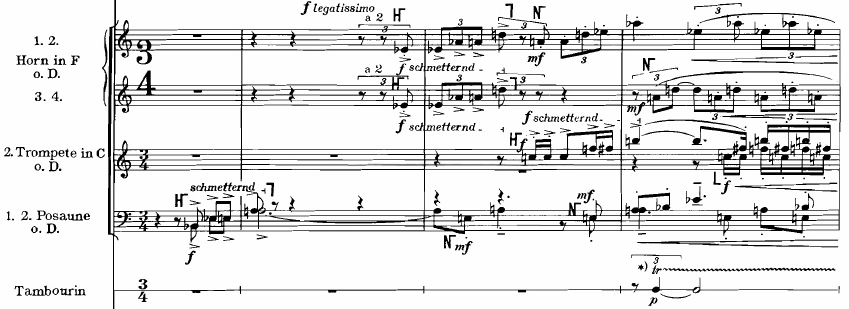
\includegraphics[width=\textwidth]{figures/berg2.png}
		\caption{Derived row in the \emph{Prologue} of Alban Berg's \emph{Lulu}.}
	\end{figure}
\end{frame}

%------------------------------------------------------------------------
\begin{frame}
	\frametitle{Derivation in Martino's \emph{Notturno}}
	\begin{block}{Example}
		Generate syntax from derivation by following $S$ with $V$ itself, then deriving a new row from $V$, say $Q$, and eventually following $V$ with $Q$. Repeating this procedure \emph{ad libitum} may generate many contrasting harmonic regions. If the chain of derived rows picked always the same order numbers, then a potential for rhythmic and agogic coherence could also be explored.
	\end{block}
\end{frame}
